% Created 2023-11-21 mar 10:54
% Intended LaTeX compiler: pdflatex
\documentclass[a4paper]{article}
\usepackage[utf8]{inputenc}
\usepackage[T1]{fontenc}
\usepackage{graphicx}
\usepackage{longtable}
\usepackage{wrapfig}
\usepackage{rotating}
\usepackage[normalem]{ulem}
\usepackage{amsmath}
\usepackage{amssymb}
\usepackage{capt-of}
\usepackage{hyperref}
\usepackage[spanish]{babel}
\usepackage[usenames,dvipsnames]{color} % Required for custom colors
\renewcommand{\ttdefault}{pcr} % MONOESPACIO CON NEGRIT
\usepackage{lastpage}
\usepackage{listings}
\usepackage{listingsutf8}
\renewcommand{\lstlistingname}{Listado}
\lstset{frame=single,inputencoding=utf8,basicstyle=\scriptsize\ttfamily,showstringspaces=false,numbers=none}
\definecolor{MyDarkGreen}{rgb}{0.0,0.4,0.0} % This is the color used for comments
\lstset{ breaklines=true, postbreak=\mbox{\textcolor{red}{$\hookrightarrow$}\space}, keywordstyle=\bfseries, keywordstyle=[1]\color{Blue}\bfseries,  keywordstyle=[2]\color{Purple}\bfseries,  keywordstyle=[3]\color{Blue}\underbar,   identifierstyle=,   commentstyle=\usefont{T1}{pcr}{m}{sl}\color{MyDarkGreen}\small,   stringstyle=\color{Purple},   showstringspaces=false,   tabsize=2,   morecomment=[l][\color{Blue}]{...} }
\lstset{literate=  {á}{{\'a}}1 {é}{{\'e}}1 {í}{{\'i}}1 {ó}{{\'o}}1 {ú}{{\'u}}1   {Á}{{\'A}}1 {É}{{\'E}}1 {Í}{{\'I}}1 {Ó}{{\'O}}1 {Ú}{{\'U}}1   {à}{{\`a}}1 {è}{{\`e}}1 {ì}{{\`i}}1 {ò}{{\`o}}1 {ù}{{\`u}}1   {À}{{\`A}}1 {È}{{\'E}}1 {Ì}{{\`I}}1 {Ò}{{\`O}}1 {Ù}{{\`U}}1   {ä}{{\"a}}1 {ë}{{\"e}}1 {ï}{{\"i}}1 {ö}{{\"o}}1 {ü}{{\"u}}1   {Ä}{{\"A}}1 {Ë}{{\"E}}1 {Ï}{{\"I}}1 {Ö}{{\"O}}1 {Ü}{{\"U}}1   {â}{{\^a}}1 {ê}{{\^e}}1 {î}{{\^i}}1 {ô}{{\^o}}1 {û}{{\^u}}1   {Â}{{\^A}}1 {Ê}{{\^E}}1 {Î}{{\^I}}1 {Ô}{{\^O}}1 {Û}{{\^U}}1   {œ}{{\oe}}1 {Œ}{{\OE}}1 {æ}{{\ae}}1 {Æ}{{\AE}}1 {ß}{{\ss}}1   {ű}{{\H{u}}}1 {Ű}{{\H{U}}}1 {ő}{{\H{o}}}1 {Ő}{{\H{O}}}1   {ç}{{\c c}}1 {Ç}{{\c C}}1 {ø}{{\o}}1 {å}{{\r a}}1 {Å}{{\r A}}1   {€}{{\euro}}1 {£}{{\pounds}}1 {«}{{\guillemotleft}}1   {»}{{\guillemotright}}1 {ñ}{{\~n}}1 {Ñ}{{\~N}}1 {¿}{{?`}}1 }
\usepackage{caption}
\usepackage{attachfile}
\usepackage[margin=1.5cm,includeheadfoot,includehead,includefoot]{geometry}
\hypersetup{colorlinks,linkcolor=black}
\usepackage{fancyhdr}
\pagestyle{fancyplain}
\chead{}
\lhead{}
\rhead{}
\cfoot{}
\lfoot{\begin{footnotesize}alvaro.gonzalezsotillo@educa.madrid.org\end{footnotesize}}
\rfoot{\begin{footnotesize}\thepage / \pageref{LastPage}\end{footnotesize}}
\usepackage[skins]{tcolorbox}
\usepackage{multicol}
\usepackage{changepage} %ajdustwidth
\usepackage{fancybox}
\usepackage{attachfile2}
\lhead{Extraordinaria 2021 (es el \\lhead)}
\rhead{Administración y Gestión de Bases de Datos (es el \\rhead)}
\lhead{Cableado de oficina}
\rhead{Planificación y Administración de Redes}
\usepackage{svg}
\usepackage{letltxmacro}
\LetLtxMacro{\originalincludegraphics}{\includegraphics}
\renewcommand{\includegraphics}[2][]{\IfFileExists{#2.pdf}{\originalincludegraphics[#1]{#2.pdf}}{\originalincludegraphics[#1]{#2}}}
\LetLtxMacro{\originalincludesvg}{\includesvg}
\renewcommand{\includesvg}[2][]{\IfFileExists{#2.pdf}{\originalincludegraphics[#1]{#2.pdf}}{\originalincludegraphics[#1]{#2.svg.pdf}}}
\usepackage{comment}
\excludecomment{NOTES}
\date{}
\title{}
\hypersetup{
 pdfauthor={Álvaro González Sotillo},
 pdftitle={},
 pdfkeywords={},
 pdfsubject={},
 pdfcreator={Emacs 28.2 (Org mode 9.6.9)}, 
 pdflang={Spanish}}
\begin{document}

\captionsetup{font=scriptsize}

\setlength{\parindent}{0em}
\setlength{\parskip}{1em}

\newtcolorbox{Aviso}[1][Aviso]{
  enhanced,
  colback=gray!5!white,
  colframe=gray!75!black,fonttitle=\bfseries,
  colbacktitle=gray!85!black,
  attach boxed title to top left={yshift=-2mm,xshift=2mm},
  title=#1
}

\newtcolorbox{cuadrito}[1][Ignorado]{
  %drop shadow southeast,
  enhanced jigsaw,
  colback=white,
}


\newcommand{\StudentData}{
  \begin{cuadrito}[1\textwidth]
    \vspace{0.3cm}
    \large{
      \textbf{Apellidos:} \hrulefill \\
      \textbf{Nombre:} \hrulefill \\
      \textbf{Fecha:} \hrulefill \hspace{1cm} \textbf{Usuario:} \hrulefill \\
    }
    \vspace{-0.2cm}
  \end{cuadrito}
}


\section{Objetivo de la práctica}
\label{sec:org0000000}
En esta práctica el alumno diseñará desde el comienzo una pequeña red de área local. Se espera que el alumno
\begin{itemize}
\item Se familiarice con los materiales necesarios para una instalación de red \emph{Ethernet}
\item Planifique y presupueste los componentes necesarios
\item Se anticipe a las necesidades de un cliente/jefe de proyecto
\end{itemize}



La última versión de este documento está accesible en \href{https://alvarogonzalezsotillo.github.io/apuntes-clase/planificacion-administracion-redes-asir1/apuntes/2/par-2-practica-cableado-oficina-guiada.pdf}{este enlace}



\section{Enunciado}
\label{sec:org0000003}
Un posible cliente pide un presupuesto para realizar la instalación de una LAN en una biblioteca.

\begin{itemize}
\item El edificio tiene 50 metros de fachada, y 60 metros de fondo.
\item El cableado vertical se aloja en el vano junto al ascensor, al lado de la fotocopiadora
\item No se dispone de suelo ni techo técnico.
\item Se desea que la fotocopiadora disponga de punto de red. Debe haber puntos de red en los tres despachos de biblioteca.
\item La sala de lectura necesita acceso wifi. Debe haber una antena a menos de 20 metros de cualquier portátil de la sala.
\item En la sala de lectura se instalarán 4 puntos de red en cada una de las 6 columnas.
\item Inicialmente, solo se espera utilizar un punto de red por cada uno de los despachos de la biblioteca, y un punto de red por columna.
\end{itemize}


\begin{center}
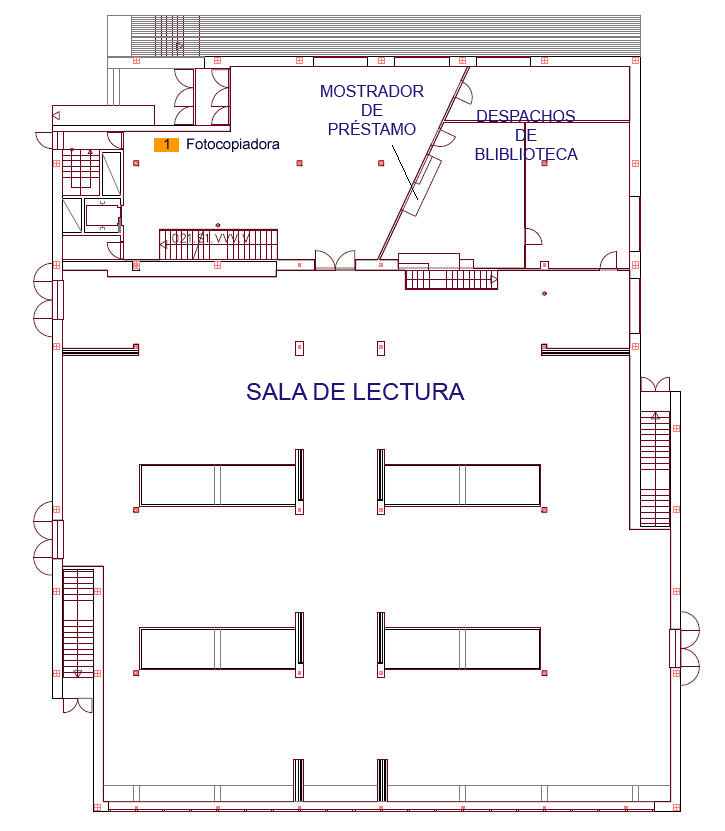
\includegraphics[width=.9\linewidth]{./media/planta-biblioteca.jpg}
\end{center}



\section{Qué se entrega}
\label{sec:org0000006}
Un documento que incluya:
\begin{itemize}
\item Planos aproximados de la situación de los puestos informáticos, puntos de red y racks
\begin{itemize}
\item Si se necesitan separaciones o tabiques, deben indicarse también.
\end{itemize}
\item Presupuesto de los materiales
\begin{itemize}
\item De red: cables, canaletas, rosetas, patch panels, switchs…
\item Desglosados por precio, cantidad, total sin IVA y total con IVA
\item Los materiales incluirán una URL o hiperlink en donde se puedan comprobar sus características y/o precio.
\end{itemize}
\item Se entregará un solo fichero en formato Microsoft Word, Open Office o PDF.
\end{itemize}



\section{Qué se valorará}
\label{sec:org0000009}
\begin{itemize}
\item 2 punto: La aplicabilidad práctica de los planos
\item 4 puntos: La completitud en la relación de materiales
\item 2 puntos: La compatibilidad de los materiales
\item 2 puntos: La apariencia profesional del trabajo
\end{itemize}


\section{Instrucciones de entrega}
\label{sec:org000000c}
\begin{itemize}
\item Se corregirá un solo documento. En él estarán embebidos todos los recursos que se quieran mostrar (explicaciones, imágenes, diagramas, tablas\ldots{})
\item El ejercicio se realizará y entregará de manera individual.
\begin{itemize}
\item Solo se admiten trabajos en pareja si en clase es necesario compartir ordenador.
\end{itemize}
\item Entrega tu trabajo en formato \textbf{doc}, \textbf{docx}, \textbf{odt} o \textbf{pdf}.
\item También puede entregarse como una entrada de blog. Para ello, sube un archivo con la URL de la entrada.
\item Sube el documento a la tarea correspondiente \href{https://aulavirtual3.educa.madrid.org/ies.alonsodeavellan.alcala}{en el aula virtual}
\item Presta atención al plazo de entrega (con fecha y hora).
\end{itemize}



\section{Guía de compras}
\label{sec:org0000018}
\subsection{Dónde realizar las compras}
\label{sec:org000000f}
\begin{itemize}
\item \url{http://www.cablematic.es}
\item \url{http://www.cablecom.es}
\item \url{http://www.senetic.es}
\item \url{http://esp.hyperlinesystems.com}
\item \url{http://www.universalnetworks.co.uk}
\item O cualquier otro sitio especializado en componentes
\item No se recomienda Amazon
\end{itemize}
\subsection{Diagrama de decisiones}
\label{sec:org0000012}
\begin{center}
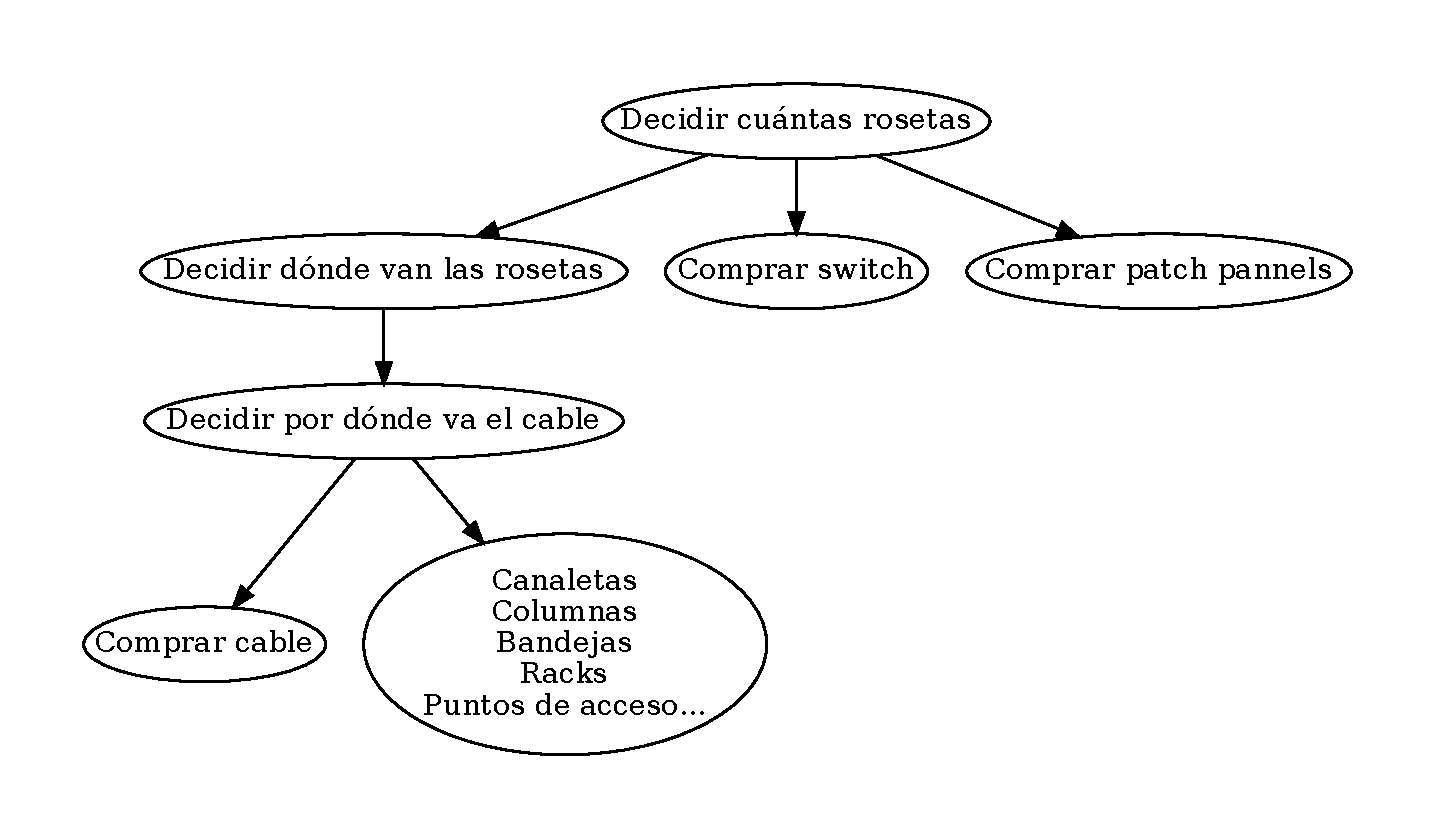
\includegraphics[width=.9\linewidth]{./media/tareas-en-la-practica.pdf}
\end{center}


\subsection{Ejemplo de posible Presupuesto}
\label{sec:org0000015}
\begin{center}
\begin{tabular}{lrrr}
Artículo con URL & Unidades & Precio unitario & Total\\[0pt]
\hline
\href{https://www.tornillos-online.com/975a2es.html}{Tornillo} & 100 & 3.60 & 360.00\\[0pt]
\href{https://www.pccomponentes.com/hp-pavilion-200-raton-gaming-3200-dpi}{Ratón} & 12 & 23.99 & 287.88\\[0pt]
Más cosas\ldots{}. &  &  & \\[0pt]
\hline
IVA 21\% &  &  & 115.05\\[0pt]
Total &  &  & 662.93\\[0pt]
\hline
\end{tabular}
\end{center}
\end{document}